\documentclass[14pt,letterpaper]{article}
\usepackage[margin=2cm,includefoot]{geometry}
\usepackage[spanish]{babel}
\usepackage[utf8]{inputenc}

\usepackage[colorlinks = true,
            linkcolor = blue,
            urlcolor  = blue,
            citecolor = blue,
            anchorcolor = blue]{hyperref}
\usepackage{amsmath}
\usepackage{graphicx}
\usepackage{listings}
\usepackage{array}
\graphicspath{ {images/} }




\title{Tarea 1}
\author{}
\date{}

\begin{document}

\ttfamily
\maketitle
\rmfamily
\begin{enumerate}
\item {\bf Instrucciones.}
  
  \item {\bf Agentes.}

    A continuación se muestra nuestro análisis de
    cada caso de acuerdo a nuestra solución:
    
    \begin{itemize}
    \item Agente Aleatorio.

      Este es el único que es no-determinista, pues
      al funcionar mediante la función {\it choice}
      el comportamiento no puede ser anticipado o
      que siempre se repita.

      En una ejecución que hicimos sucede los siguiente:

      %% Imagen
      \begin{centering}
        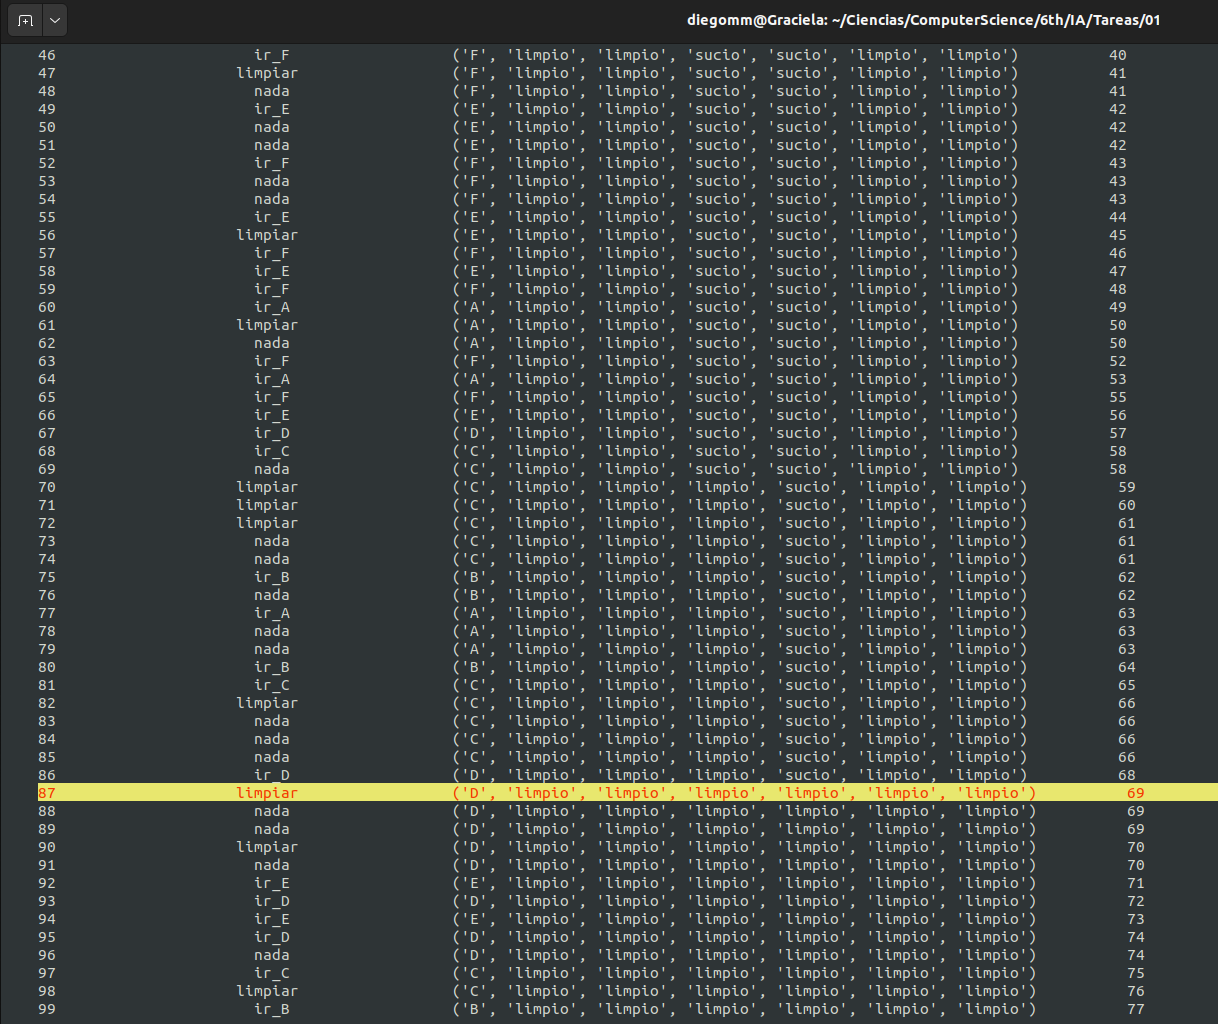
\includegraphics[scale=.3]{aleatorio}
      \end{centering}
      
      Nuestro agente termina de limpiar
      los seis cuartos en la iteración/decisión 87
      y con un costo de 69 y terminando las cien
      iteraciones con un costo de 77.

      Las cien iteraciones pueden o no ser suficientes
      para limpiar los sesis cuartos, así que no podriamos decir
      que funciona de una manera optima.
      \newpage
    \item Agente reactivo Simple.

      Al igual que el siguiente agente este es determinista
      y lo que hace es comenzar en A, para el cuarto en el que se encuentre
      si el estado es sucio procede a limpiar y si no no importa el cuarto
      en la que se encuentre se mueve haciendo un ``circulo'' hacia la derecha,
      es decir siguiendo el recorrido:

      $$ A\rightarrow B \rightarrow C \rightarrow D \rightarrow E \rightarrow F \rightarrow A ...$$

      %% Imagen
      \begin{centering}
        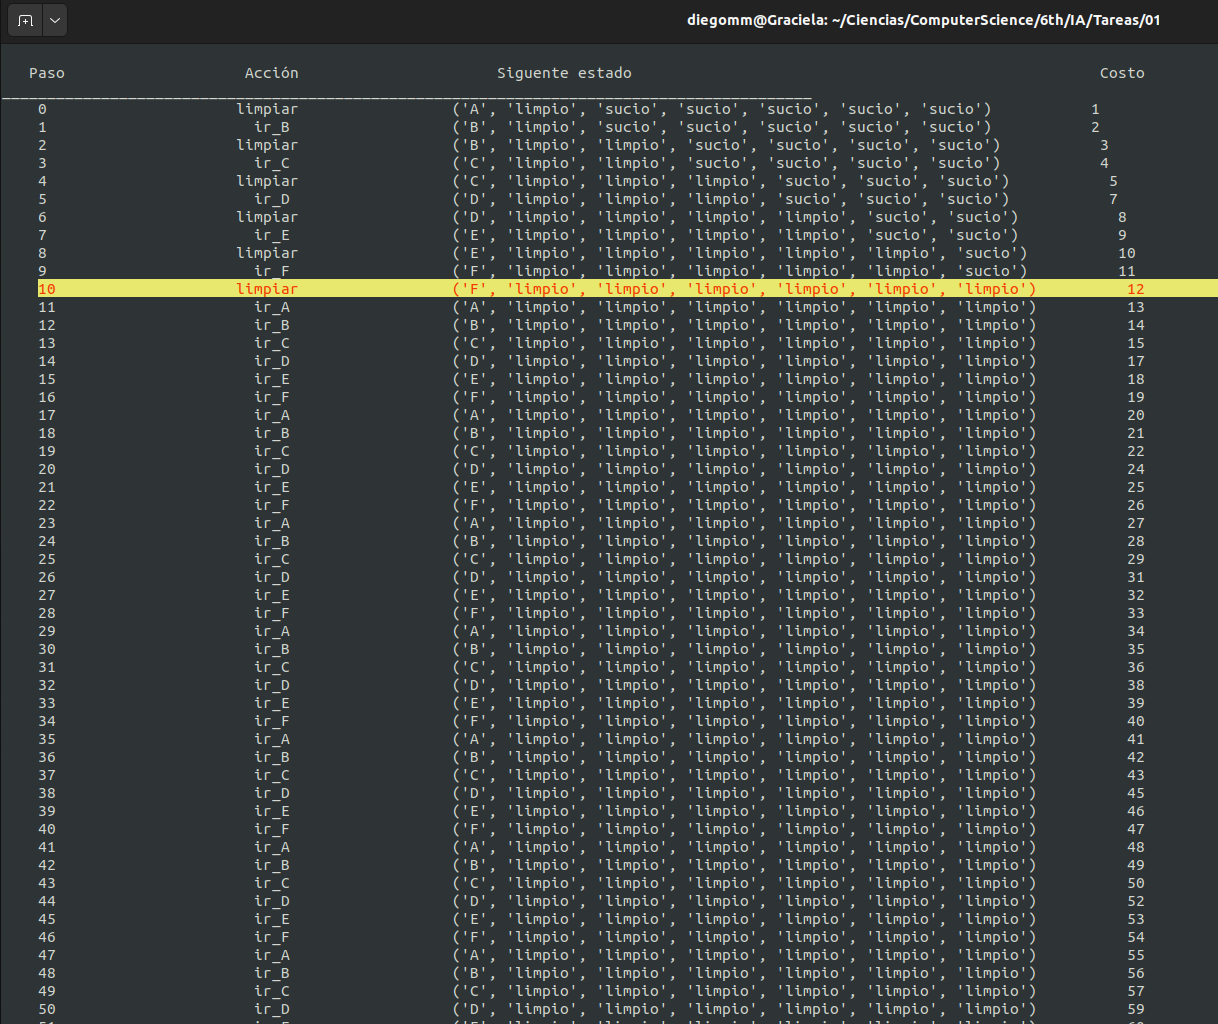
\includegraphics[scale=.3]{simple}
      \end{centering}

      Vemos que para la decima iteración los seis cuartos se encuentran limpios con un costo
      de 12,  pero al ser simple y solo reaccionar a lo que se encuentra nunca para
      su recorrido y lo perpetua durante las cien iteraciones. Terminando
      con un costo de 116. Pareciera ser más optimo en el tiempo en el que
      limpia pero como nunca descansa el costo al final {\it puede} ser peor
      que el del aleatorio.     
      \newpage      
    \item Agente reactivo con Modelo.

      Para este solo faltaba optimizar lo restante del agente anterior,
      que es hacer que nuestro robot se pare en cuanto haya limpiado todos los cuartos.
      En la vida real quiza habria que programarlo para escanear los cuartos en busca de
      algún sucio o poder informarle mediante una aplicación que cierto cuarto
      se ensució.

      %% Imagen
      \begin{centering}
        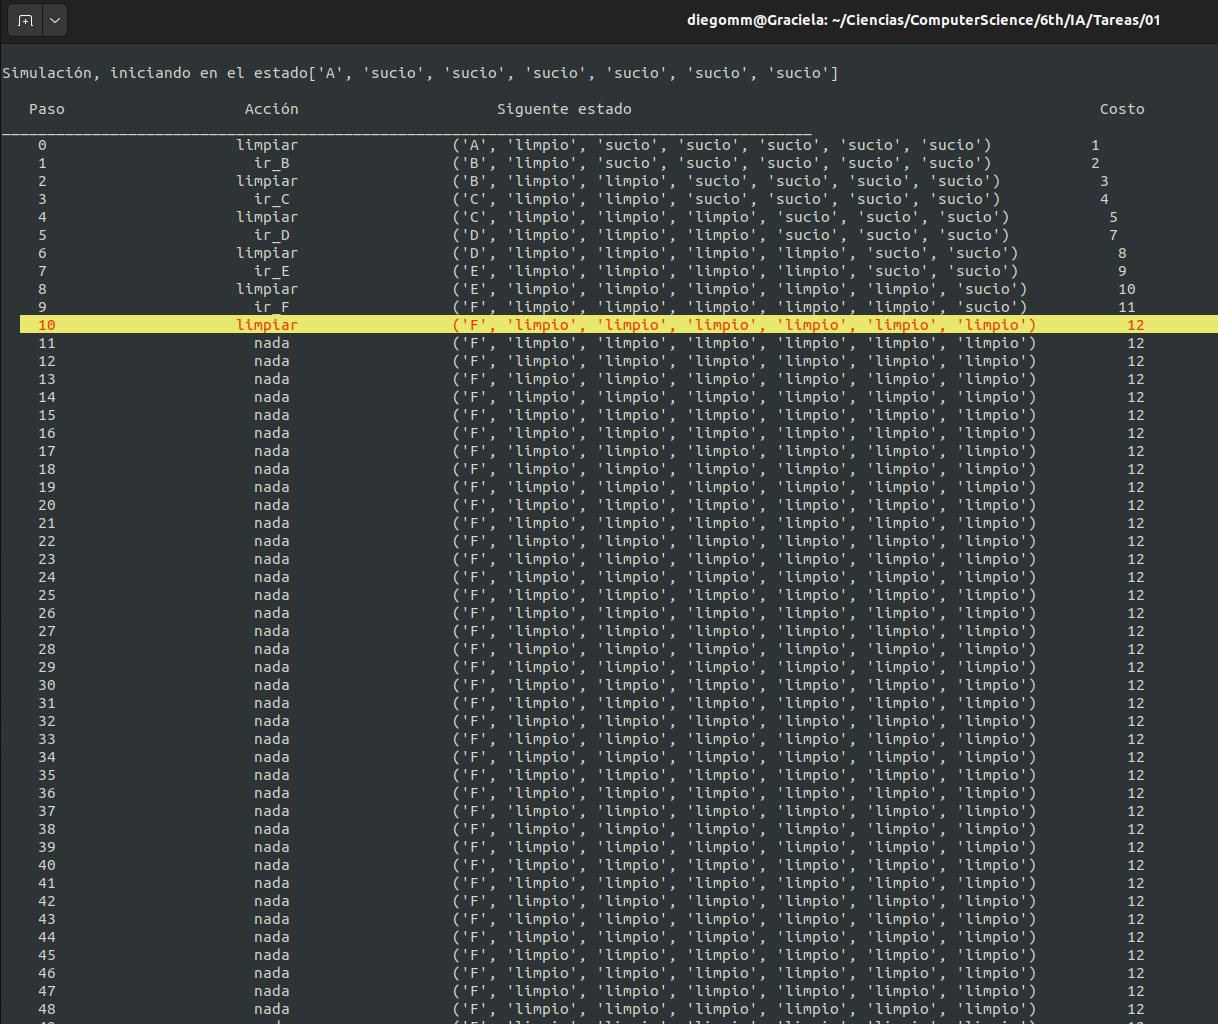
\includegraphics[scale=.3]{modelo}
      \end{centering}
      
      Tambíen termina en la decima iteración, pero de ahí en adelante ya no
      hace nada es decir no genera costo.
    \end{itemize}
    
  \item {\bf Búsqueda Ciega.}

    La implementación se encuentra en el archivo {\it tarea\_1.py} y al
    ejecutarlo se corre sobre la gráfica solicitado. El resultado se muestra
    en la salida standard despúes de la sección de los agentes.

    Nuestra ejecución devuelve el siguiente topological sort:

      %% Imagen
      \begin{centering}
        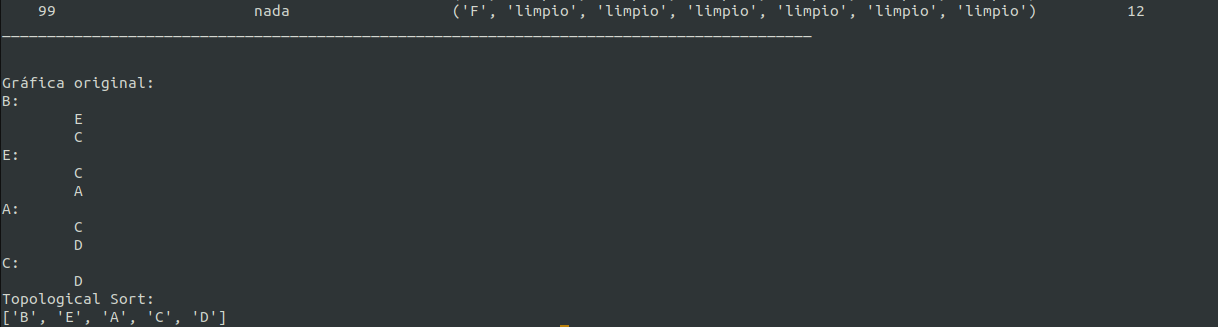
\includegraphics[scale=.3]{topological_sort}
      \end{centering}

      Que cumple con lo recorrido.
  \item {\bf Búsqueda Informada.}
  \end{enumerate}
\end{document}
